



\chapterimage{Chapter11.jpg} % Chapter heading image

\chapter{Nutrient Removal}

\section{Importance of removing nutrients}\index{Importance of removing nutrients}
\begin{itemize}
\item Plant nutrients - nitrogen and phosphorous, if present in wastewater effluent discharge promote growth of plant and algal matter in the receiving waters causing destruction of the normal aquatic life mainly due to oxygen depletion - eutrophication.

\item Because of the potential impacts of the presence of these nutrients in wastewater effluent on the receiving waters,  limits on the levels of these nutrients is typically stipulated in the treatment plant's wastewater discharge permit.

\item Typically, conventional secondary treatment processes are designed primarily remove the organics from the wastewater.  Secondary treatment process designed to additionally remove nutrients is deemed as tertiary or advanced treatment is termed as Biological Nutrient Removal (BNR).
\end{itemize}

\section{Nitrogen Removal}\index{Nitrogen Removal}

Nitrogen exists in many forms and changes from one form to another in the environment as part of the nitrogen cycle below.

	\begin{itemize}
		\item In raw domestic wastewater, nitrogen exists primarily as organic nitrogen (40\%) and ammonia nitrogen (60\%). 
		\item The sum of organic nitrogen and ammonia nitrogen is referred to as “Total Kjeldahl Nitrogen” (TKN).  
		\item The important forms of nitrogen as part of wastewater treatment are: N$_2$ (Nitrogen Gas), NO$_2^{\enspace -}$ (Nitrite), NO$_3^{\enspace -}$ (Nitrate), NH$_3$ (Ammonia), NH$_4^{\enspace +}$ (Ammonium Ion), and Organic Nitrogen. 
	\end{itemize}
%\floatstyle{boxed} 
%\restylefloat{figure}
\begin{figure}[h]
	\begin{center}
	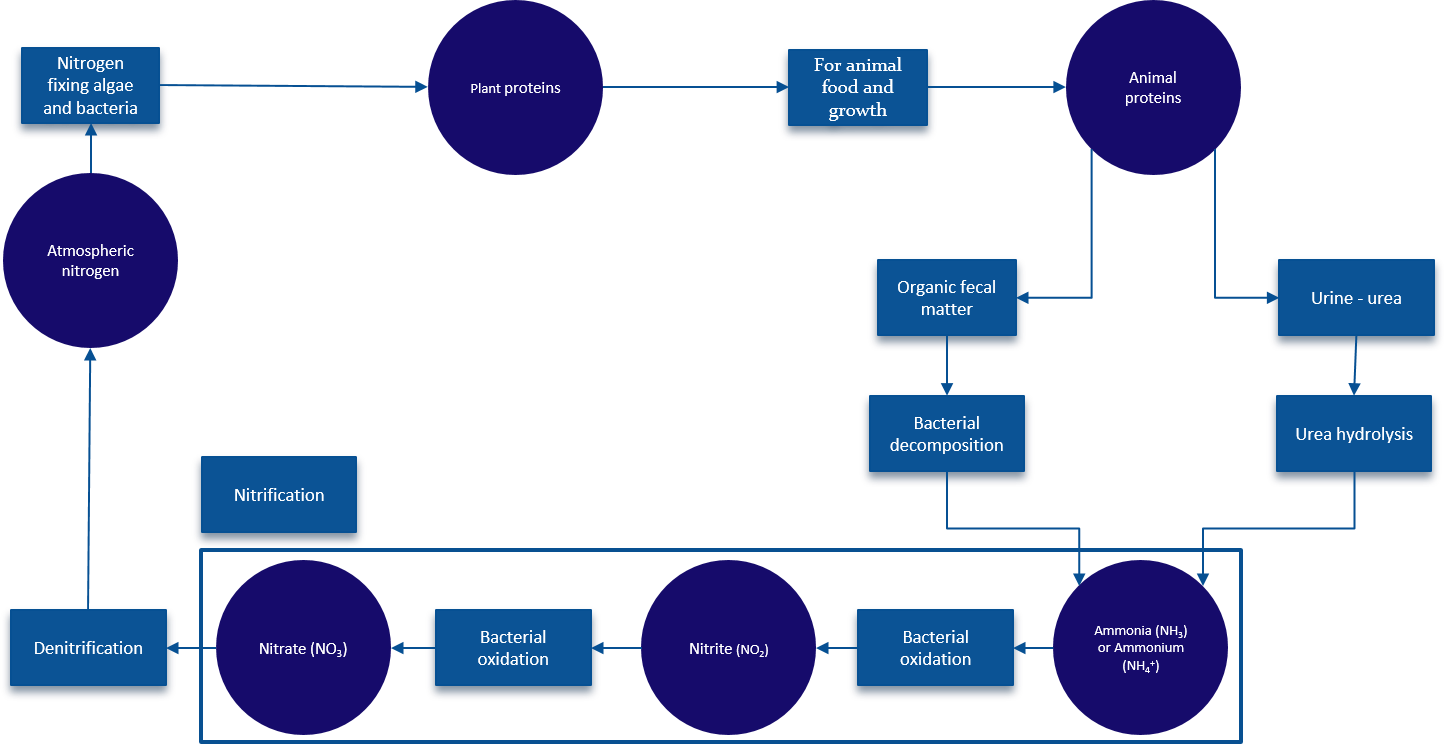
\includegraphics[scale=0.6]{NitrogenCycle}
	\caption{Nitrogen Cycle}
		\end{center}
\end{figure}

	Typical concentrations of the nitrogen constituents in wastewater are tabulated below.\\

\setlength{\arrayrulewidth}{0.6mm}
\setlength{\tabcolsep}{8 pt}
\renewcommand{\arraystretch}{1.2}
	\begin{center}
	\begin{table}
		%{\rowcolors{3}{green!60!yellow!50}{green!30!yellow!40}
		\begin{tabular}{ |p{6.5cm}|p{2.0cm}|p{2.5cm}|p{2.5cm}|}
			\hline
			\multicolumn{4}{|c|}{\textbf{NITROGEN IN WASTEWATER}} \\
			\hline
			%\thead{A Head} & \thead{A Second \\ Head} & \thead{A Third \\ Head} \\
			%\hline%

			\hspace{1.8 cm}Forms of Nitrogen & \hspace{0.25 cm} Formula & \hspace{.4 cm} Found in & \hspace{.4 cm} Typical \newline \hspace{.2 cm}Concentration\\
			\hline
			\small Ammonia/Ammonium & \small NH$_3$/NH$_4^{\enspace +}$ &  \small Influent wastewater & 30-50 mg/l\\

			\small Total Kjeldahl Nitrogen \newline  \small (Ammonia/Ammonium + Organic Nitrogen) &  \small TKN &  \small Wastewater \newline  \small effluent  & 30-60 mg/l \\

			 \small Total Inorganic Nitrogen \newline  \small (Ammonia/Ammonium + Nitrite + Nitrate) & \small TIN &  \small  Wastewater \newline  \small effluent  & 1-40 mg/l \\

			 \small Nitrate  & $NO_3^{\enspace -}$ &  \small Nitrified effluent &  \small 1-35 mg/l \\

			 \small Nitrate  &  $NO_2^{\enspace -}$ &  \small Partially nitrified effluent &  \small 0.1-2 mg/l \\

			\hline

		\end{tabular}
					\caption{Forms of Nitrogen in Wastewater}
		\end{table}
		
	\end{center}
Ammonia (NH$_3$) and ammonium (NH$_4^+$) are both commonly referred to as “Ammonia-nitrogen (NH$_3$-N)” These two forms of nitrogen can rapidly change from one to the other depending on pH and temperature. The figure below illustrates the relative distribution of ammonia (unionized ammonia) and the ammonium ion (ionized ammonia)in water as a function of pH.\\

\begin{figure}
	\begin{center}
		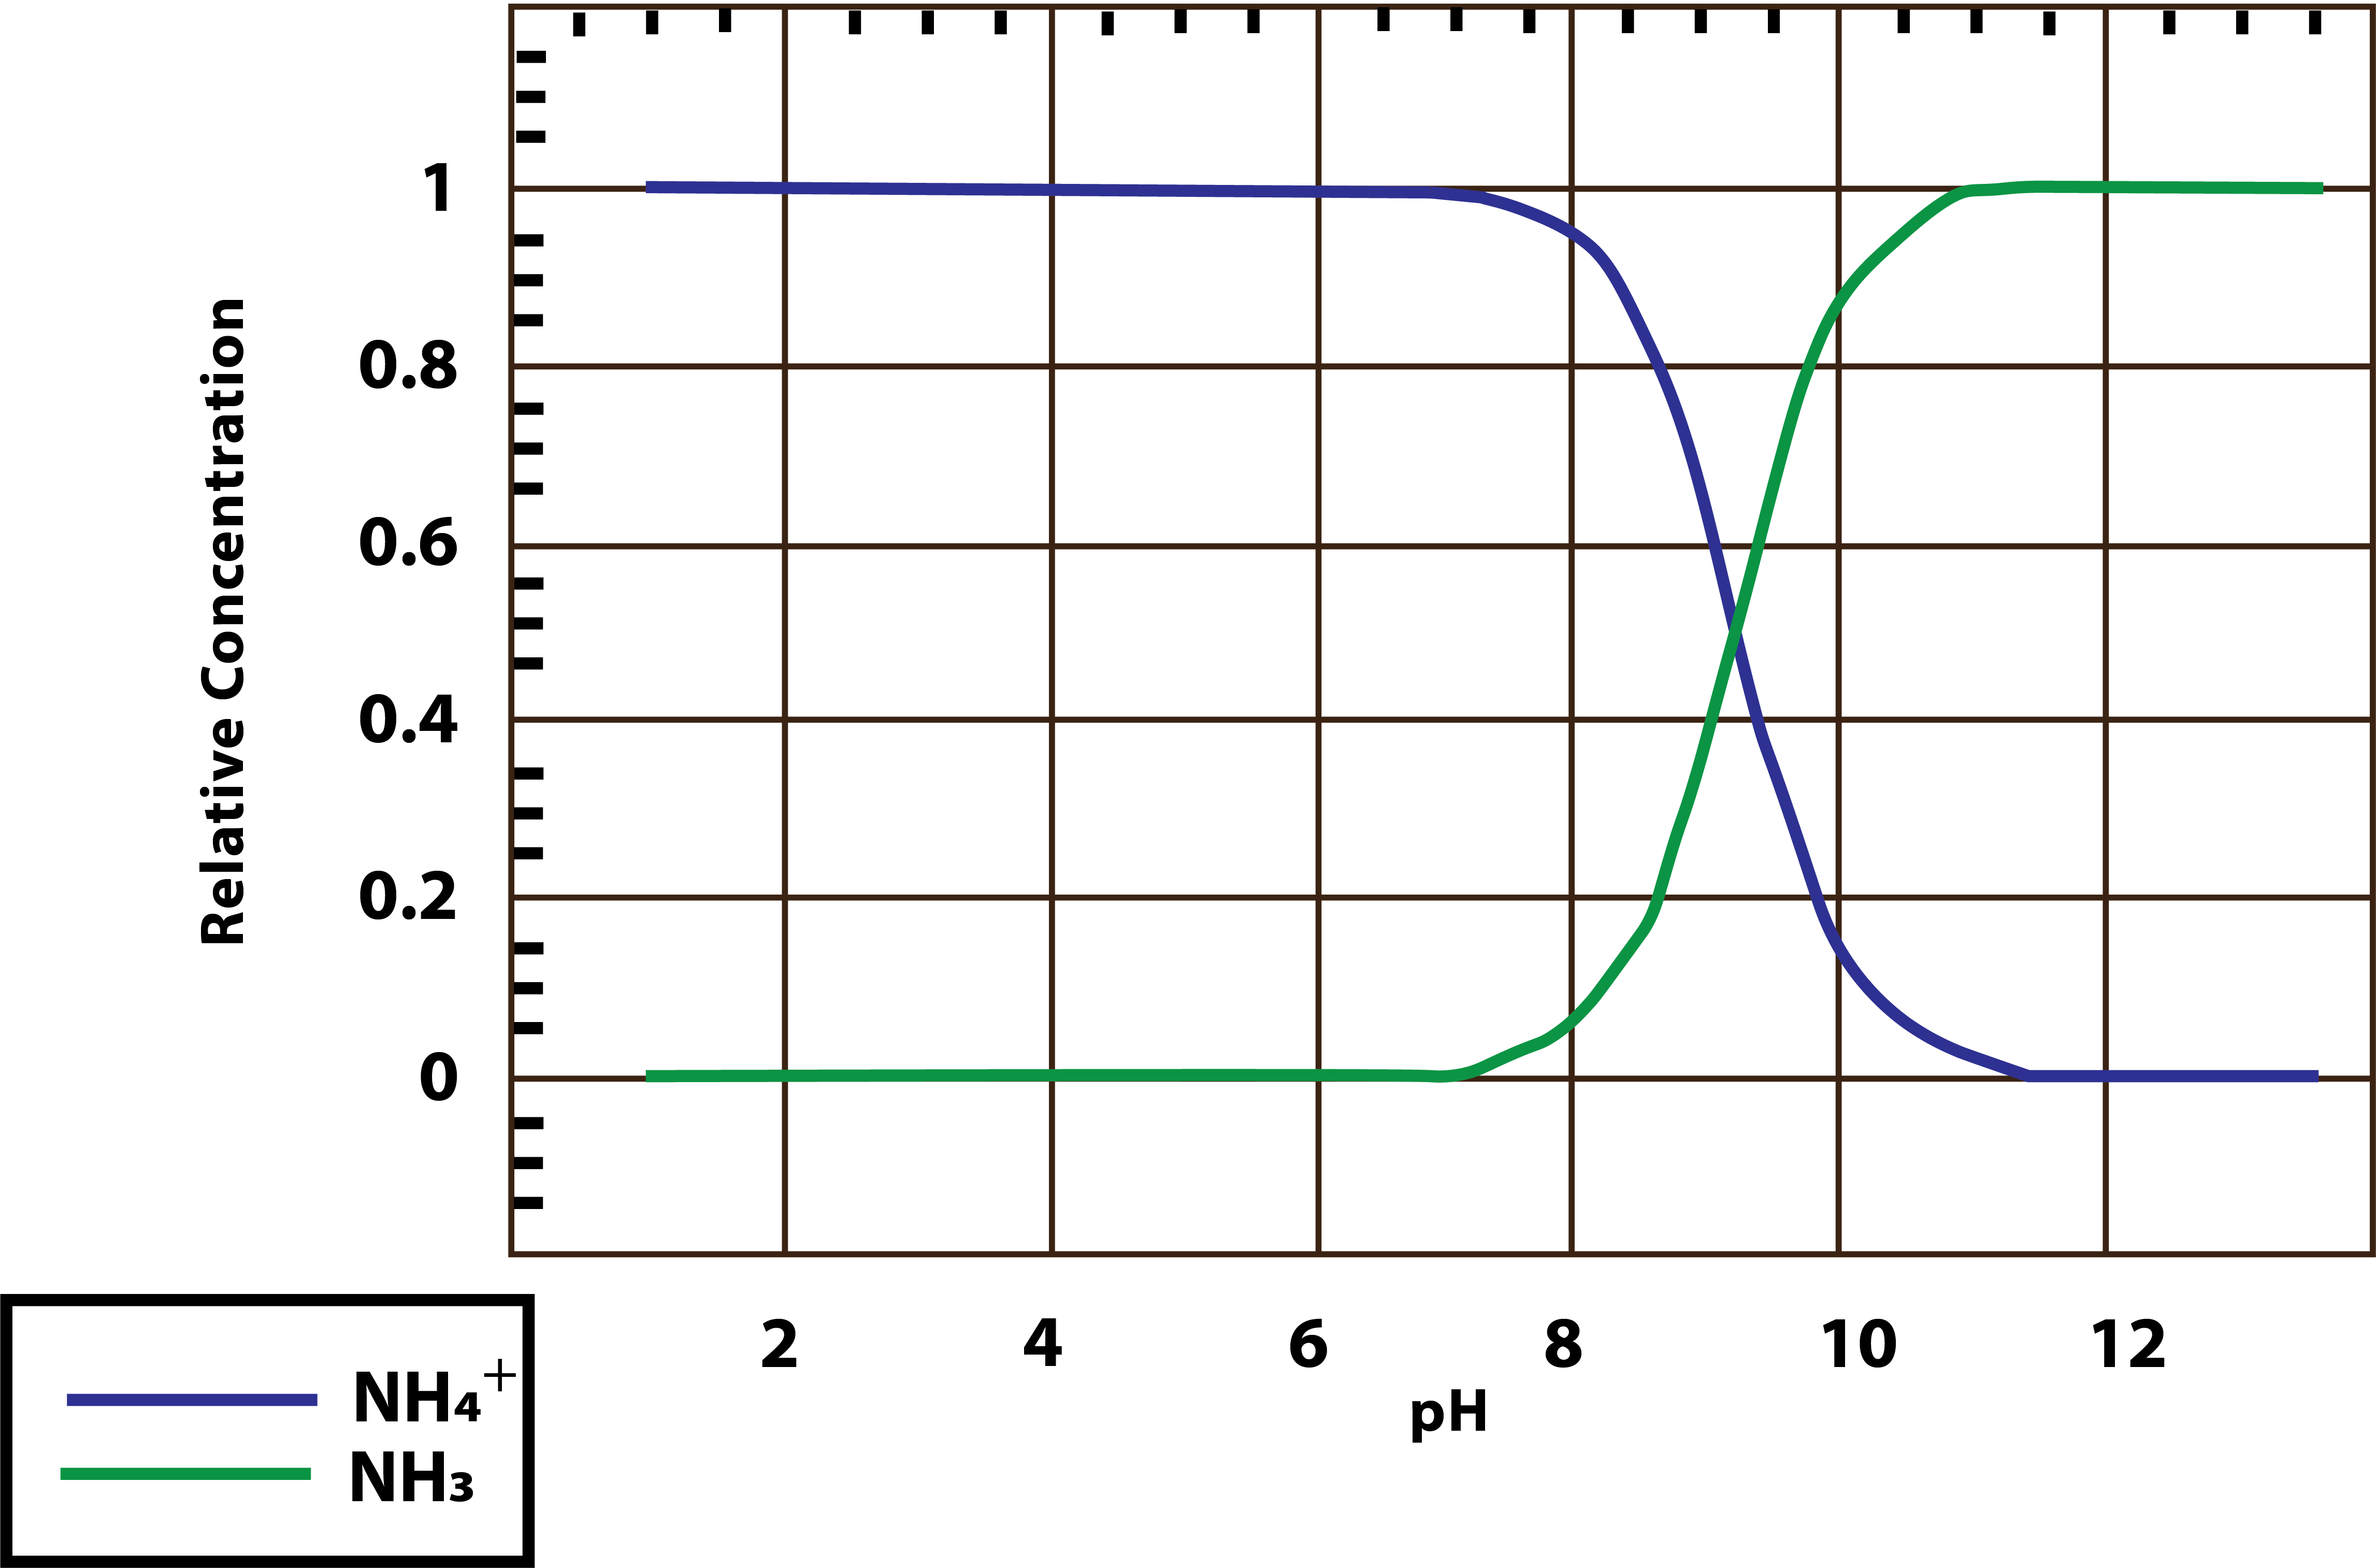
\includegraphics[scale=.35]{AmmoniaAmmoniumEquilibrium}
			\caption{Ammonia-Ammonium Equilibrium}
	\end{center}
	
	\end{figure}
	\begin{itemize}
		\item In biological treatment processes, the organic nitrogen is quickly changed to ammonia nitrogen by natural processes.
		\item Ammonia-nitrogen is toxic to aquatic life and toxicity is affected by both, temperature and pH of water. 
			\begin{itemize}
				\item Toxicity of ammonia nitrogen increases as temperature increases
				\item Ammonia nitrogen is toxic when present as unionized NH$_3$.  This unionized ammonia NH$_3$ is the predominant form of ammonia nitrogen at higher pH.  The ammonia nitrogen (NH$_3$-N)toxicity is lower when present as  ionized ammonia (NH$_4^+$)
			\end{itemize}
	\end{itemize}
	\vspace{0.3cm}
	
	\subsection{Nitrogen Removal Methods}\index{Nitrogen Removal Methods}
	
		\subsubsection{Nitrification and denitrification}\index{Nitrification and denitrification}

This is the most common ammonia removal process and is accomplished during secondary treatment.  It is a two-step process:
			\begin{enumerate}
				\item \textbf{Nitrification} This involves conversion of ammonia to nitrate
				\item \textbf{Denitrification} This involves conversion of nitrate to gaseous nitrogen which escapes from the waster.
			\end{enumerate}


\noindent\textsc{{Nitrification}}%$$$$$$$$$$$$$$$$$$$$%

			\noindent Nitrification is a two step process:
			
			Step 1:  Nitrosomonas and other similar bacteria oxidizes ammonium to nitrite via hydroxylamine.
			$$2NH_4^{+} + O_2 \rightarrow 2NH_2OH + 2H^{+}$$
			$$NH_4^{+} + 1.5 O_2 \rightarrow NO_2^{\enspace -} + 2H^{+}+ H_2O$$
					 
			Step 2:  Conversion of nitrite to nitrate by nitrobacter and other similar bacteria
			$$NO_2^{\enspace -} + 0.5O_2 \rightarrow NO_3^{\enspace -}$$

			\begin{itemize}
				\item The above two reactions are generally coupled and precede rapidly to the nitrate form; therefore, nitrite levels at any given time are usually below 0.5 mg/L.
				\item Nitrifiers (responsible for the consumption of nBOD) compete with the organotrophs which consume the cBOD in the secondary reactor.  \item Nitrification occurs at the tail end of the secondary treatment reactor when the cBOD is low and the organotrophs are not as active
				\item Nitrification occurs 3-4 times slower than carbonaceous oxidation
				\item For nitrosomonas to generate 1 part of new cells it needs 30 parts of ammonium ions and nitrobacter needs 100 parts of nitrite ions to generate 1 part new cells.  Due to the high demand of the nitrogen based ions, the reproductive rates of nitrifiers are very low thus plant upsets can take nitrifiers weeks to recover as opposed to days or hours for carbon bacteria.  
				\item For each 1-gram of NH$_3$-N oxidized to NO$_3$, 0.15 grams of new bacteria cells are formed.  Sludge generation from nitrifiers is minimal in a wastewater treatment plant.
			\end{itemize}
				Controlling Factors for Nitrification:
			\begin{enumerate}
				\item Dissolved oxygen
				\noindent Oxygen levels are critical for nitrification. Higher levels of oxygen are required for nitrification than for carbon removal.  While 1 part of O$_2$ is needed for removing 1 part of cBOD, 4.5 parts of O$_2$ are needed for every part of NH$_4^{\enspace +}N$ (nBOD) to be degraded. In order for nitrification to occur, dissolved oxygen levels of 1.0 to 4.0 mg/L are usually maintained in the aeration tanks.  Maximum nitrification occurs at DO levels of about 3.0 mg/L.  Nitrification will therefore result in significantly higher power cost due to the needs for maintaining the higher oxygen level
				\item Alkalinity and pH

				\noindent \textbf{Nitrification leads to a depletion of alkalinity in the activated sludge mixed liquor.}  Nitrosomonas and Nitrobacter use carbonate as their carbon (food) source and the ammonia is just their energy transfer source.  As the total alkalinity of wastewater is due to the individual contributions of carbonate, bicarbonate and hydroxide ions, consumption of carbonate and bicarbonate ions by the nitrifiers results in the depletion of alkalinity.  Alkalinity provides a buffer for pH change.  If the alkalinity is reduced beyond certain levels, further formation of acidic metabolic byproducts of bacterial activity may lead the pH to decline inhibiting bacterial activity. \textbf{7.14 parts of alkalinity are required for each part of ammonia removed.}    Nitrification rates are rapidly depressed as the pH is reduced below 7.0. pH levels of 7.5 to 8.5 are considered optimal.  That is why alkalinity is extremely critical in nitrification.  An alkalinity of 60 mg/L in the secondary treatment reactor (aeration tank, trickling filter, RBC, etc.) is generally required to ensure adequate buffering
	 			\item MCRT, F/M, or Sludge Age
				\noindent \textbf{For nitrification to occur the activated sludge treatment process needs to be operated at higher MCRT as the reproductive rates of nitrfiers is low.}  An MCRT of greater than 8 days is typically considered essential for nitrification to occur.
				\item Wastewater temperature
				\noindent \textbf{Nitrification is inhibited at lower wastewater temperatures in wastewater treatment plants.} To achieve the same level of nitrification, longer detention time may be needed in the winter versus the summer months since the activity drops significantly.  Lower temperature effects on Nitrification may be partially mitigated by increasing MLVSS and MCRT.  The optimal temperature range for nitrification is between 60$^{\circ}$  to 95$^{\circ}$  degrees F. Below 40$^{\circ}$  nitrification will probably not occur.
	
\floatstyle{boxed} 
\restylefloat{figure}
		\begin{figure}
				\begin{center}
					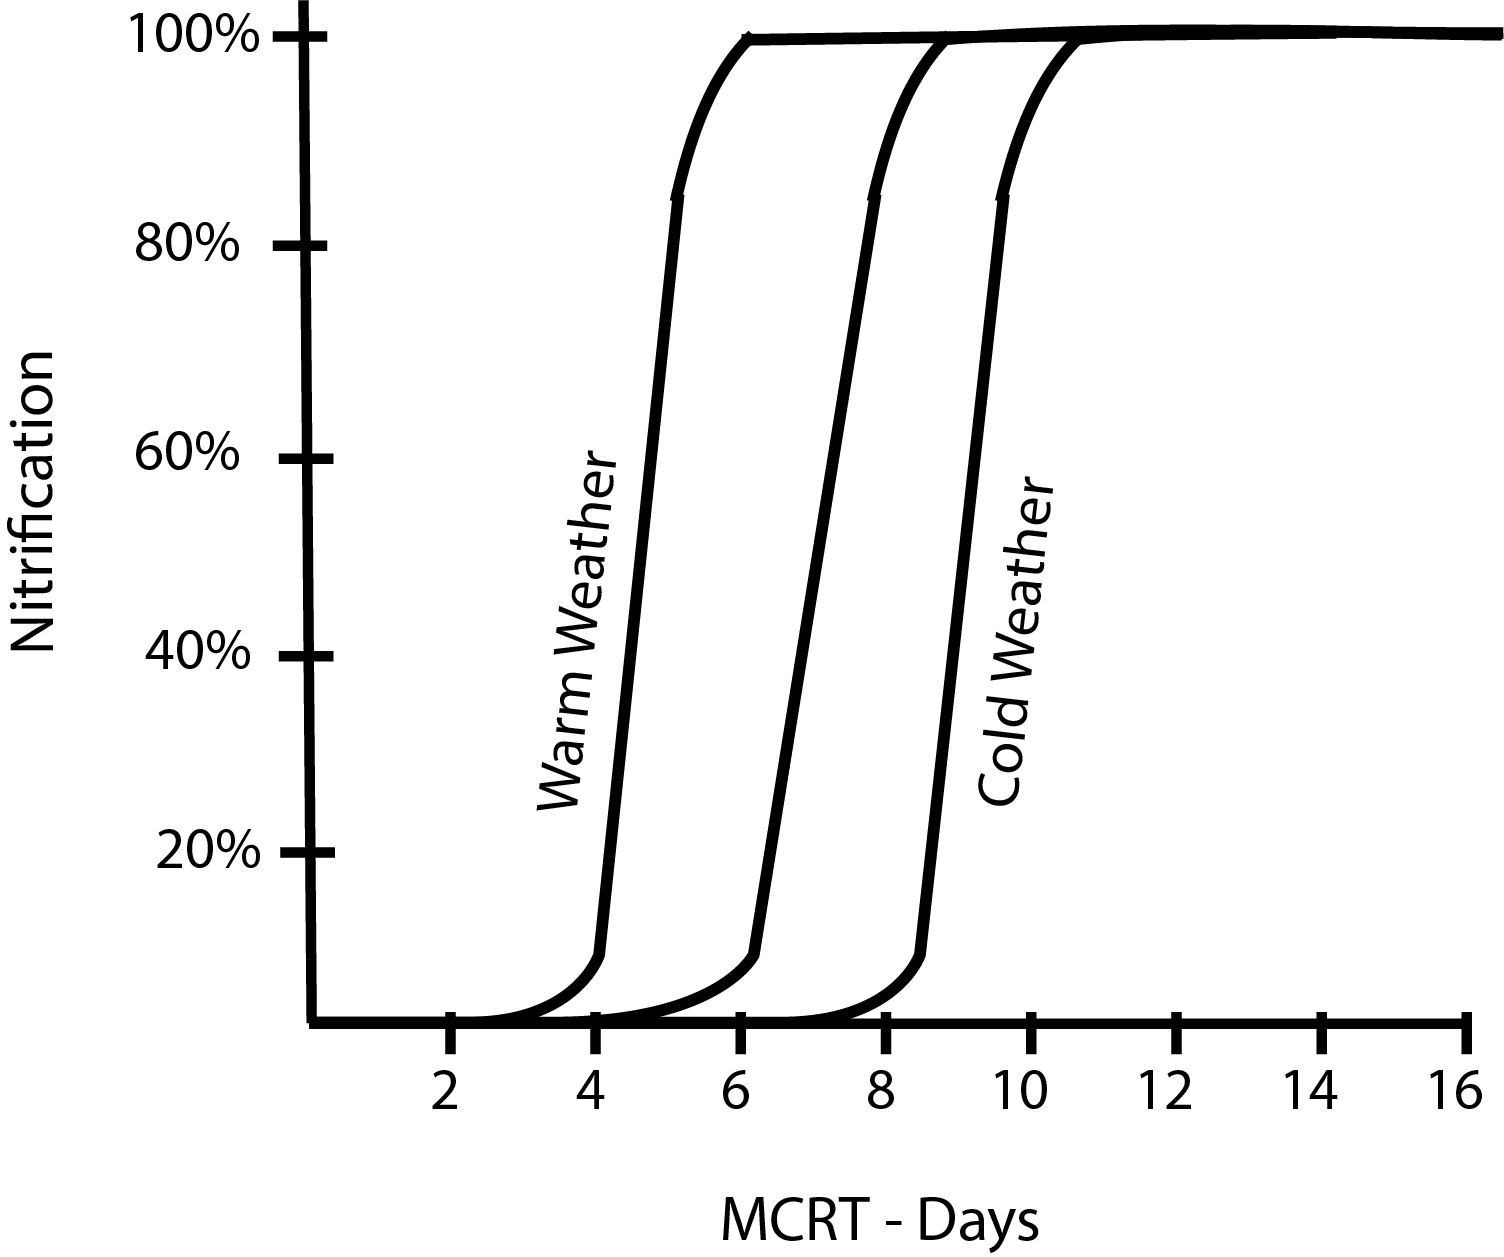
\includegraphics[scale=0.6]{NitrificationCurve}
								\caption{Weather Effects on MCRT Requirements for Nitrification}
				\end{center}
		\end{figure}
				\item Inhibition to nitrification by toxic compounds
				\noindent Many compounds can be toxic to nitrifiers- Nitrosomonas and Nitrobacter.  These include unionized ammonia, heavy metals, solvents and cyanide.  
			\end{enumerate}
			\newpage
\noindent\textsc{{Denitrification}}%$$$$$$$$$$$$$$$$$$$$%
			\begin{itemize}
				\item Dentrification is a microbiological process in which the nitrate formed during nitrification is reduced by bacteria in anoxic conditions to molecular nitrogen which is insoluble in water and escapes into the atmosphere.
				\item A large percentage of the bacteria in the activated sludge process are capable of denitrification. In the absence of free molecular oxygen – under anoxic conditions, these bacteria present in the activated sludge process utilize the nitrate and nitrite to degrade the cBOD.  
				$$NO_3^- + cBOD   \rightarrow NO_2^- + CO_2 + H_2O$$
				$$NO_2^- + cBOD   \rightarrow N_2 + CO_2 + H_2O$$
				\item Approximately 50\% of the alkalinity lost during nitrification is recovered during denitrification.  
				\item The quantity of cBOD available is critical for denitrification to occur.  Complete denitrification usually occurs at a cBOD to nitrate and nitrite ratio of approximately 3:1. Given the need for the presence of adequate cBOD for the denitrification step, a cBOD supplement (a suitable organic compound - example: alcohol) is utilized in certain configurations.  
				\item If the aeration reactor effluent is nitrified, denitrification can occur in clarifier.  The absence of aeration in the clarifier creates anoxic conditions which makes the condition favorable for denitrification to occur.  Denitrification in the secondary clarifier is not desirable as the nitrogen evolved will cause the sludge settling in the clarifier to rise to the surface.
			\end{itemize}
			\noindent Three of the more common methods to denitrify the nitrified effluent are:\\
			\vspace{0.3cm}
\noindent \textbf{Method 1.}The aeration tank is followed by a denitrifying tank which is not aerated but is supplied with organic substrate (cBOD source) such as methanol or acetic acid.  
				
	\begin{figure}[h]			
				\begin{center}
					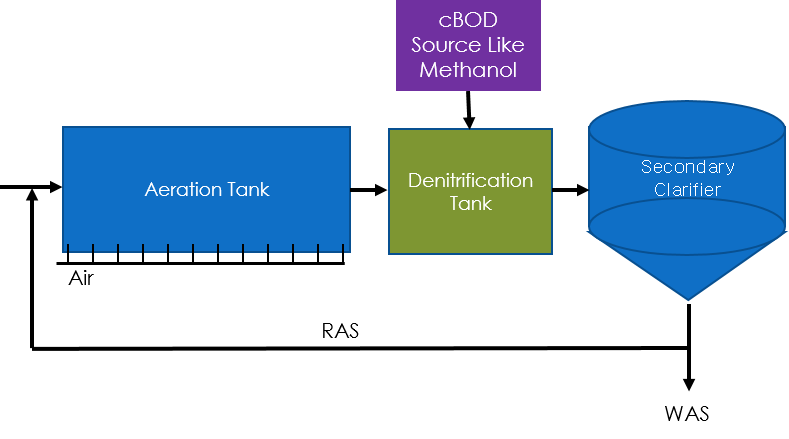
\includegraphics[scale=0.8]{Option1}
					\caption{Denitrification Method 1:\\Organic substrate addition}
				\end{center}
	\end{figure}	
\noindent \textbf{Method 2.}The mixed liquor along with RAS is recirculated to an anoxic zone at the inlet of the aeration tank where it is mixed with the influent.  The anoxic zone has mixing provided but no aeration.  The influent flow provides the necessary cBOD for the denitrification process.\\

			\begin{figure}[h]	
				\begin{center}
					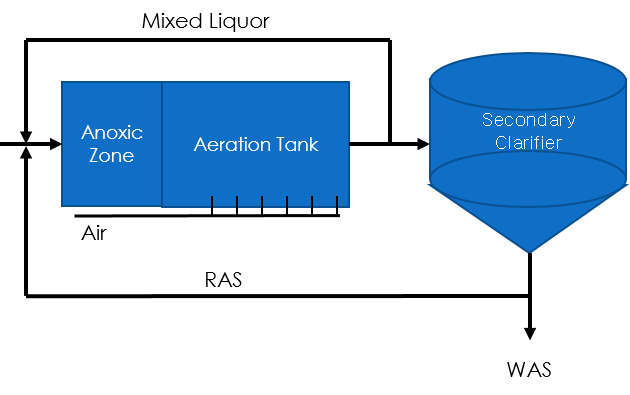
\includegraphics[scale=0.8]{Option2}
					\caption{Denitrification Method 2:\\Mixed liquor recirculation}
				\end{center}
					\end{figure}
					\newpage
\noindent \textbf{Method 3.}The aeration tank consists of alternating oxic (aerated) and anoxic zones
				
			\begin{figure}[h]		
				\begin{center}
					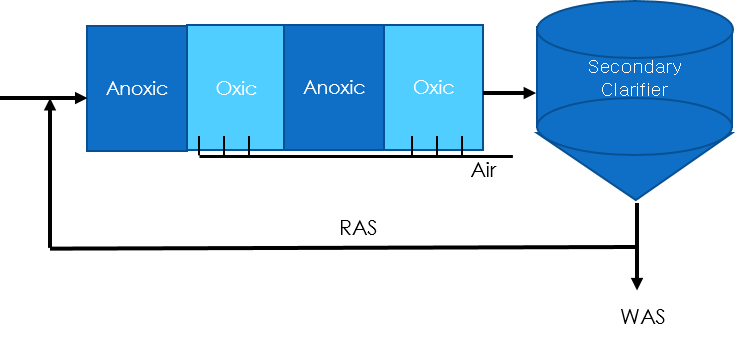
\includegraphics[scale=0.8]{Option3}
			\caption{Denitrification Method 3:\\Alternating oxic-anoxic zones}
				\end{center}
				\end{figure}

\subsubsection{Breakpoint chlorination}\index{Breakpoint chlorination}
			\begin{itemize}
				\item Breakpoint chlorination is a means of eliminating ammonia using chlorine
				\item As chlorine is added to water containing ammonia, it converts ammonia into chloramines which in the presence of additional free chlorine forms nitrogen gas which is released to the atmosphere
			\end{itemize} 
Chlorination of a water containing ammonia results in the following:
			\begin{itemize}
				\item an initial increase in combined chlorine residual
				\item followed by a decrease in the combined chlorine residual
				along with ammonia concentrations
				\item followed by an increase in free chlorine residual and near complete removal 					of ammonia as nitrogen gas.\\
				\item Chlorine reacts with ammonia to form chloramines\\
				\begin{enumerate}
					\item First the free chlorine in contact with ammonia forms monochloramine and water
						\begin{itemize}
							\item Monochloramine has disinfection properties\\
							\item Dominates when Cl:N mass ratio is 0 to 5:1\\
							\item The breakpoint curve rises at about 1:1 during monochloramine formation\\
						\end{itemize}
					$NH_3 + HOCl   \rightarrow NH_2Cl (monochloramine) + H2O$\\
					\item Monochloramine reacts further with chlorine to give dichloramine and water\\
					$HOCl + NH_2Cl \rightarrow NHCl_2 + H_2O$\\
					Also, monochloramine auto decomposes into dichloramine\\
					$2NH_2Cl \rightarrow NHCl_2 + NH_3$
						\begin{itemize}
							\item Between dichloramine is formed between 5:1 and 7:1 Cl:N mass ratio
							\item When you are getting significant dichloramine, the breakpoint curve will start dropping
						\end{itemize}
						$NH_2Cl + HOCl  \rightarrow NHCl_2 (dichloramine)$\\
						at pH $>$ 7.5, monochloramine is the dominant chloramine species as pH decreases from 7.5, dichloramine becomes the dominant chloramine species increases in the chlorine to nitrogen dose ratio results in corresponding increases of nitrogen trichloride, but only when the pH is $<$ 7.4\\
					\item Formation of nitrogen trichloride from the reaction of chlorine and dichloramine does not typically occur as it is the favored product at low pH - $<$4\\
					$NHCl_2 + HOCl  \rightarrow NCl_3 (nitrogen trichloride)$\\
					\item Additional $free \enspace chlorine \enspace + chloramines \enspace \rightarrow H^+ + H2O + N_2$
				\end{enumerate}
				\item Chloramines have disinfection properties albeit much lower than free chlorine (~5\% of free available chlorine) but last much longer in the system than free chlorine. 
				\item After the breakpoint, free chlorine residuals develop. Free chlorine residuals usually destroy odors, kill microorganisms and oxidize organic matter.
				\item Breakpoint chlorination is the application of sufficient chlorine beyond the chlorine demand to maintain a free available chlorine residual.\\  Theoretically chlorine requirement = Wt. NH$_3$-N x 7.6\\
				in practice (Margin of safety)     = Wt. NH$_3$-N x 10\\
				\item Thus, breakpoint chlorination is possible if ratio of Cl$_2$ to ammonia exceeds 10:1 then free Cl$_2$ may exist. Cl$_2$ demand will be high because the reaction of free Cl$_2$ with nitrite and other organic compounds. 
				\item Theoretically, while microorganisms are killed as the chlorine demand is being satisfied, disinfection is generally the result of chlorine residual or the amount of chlorine remaining after the chlorine demand has been satisfied.
			\end{itemize}
The following chart is a graphical explaination of the concept of Breakpoint Chlorination\\
			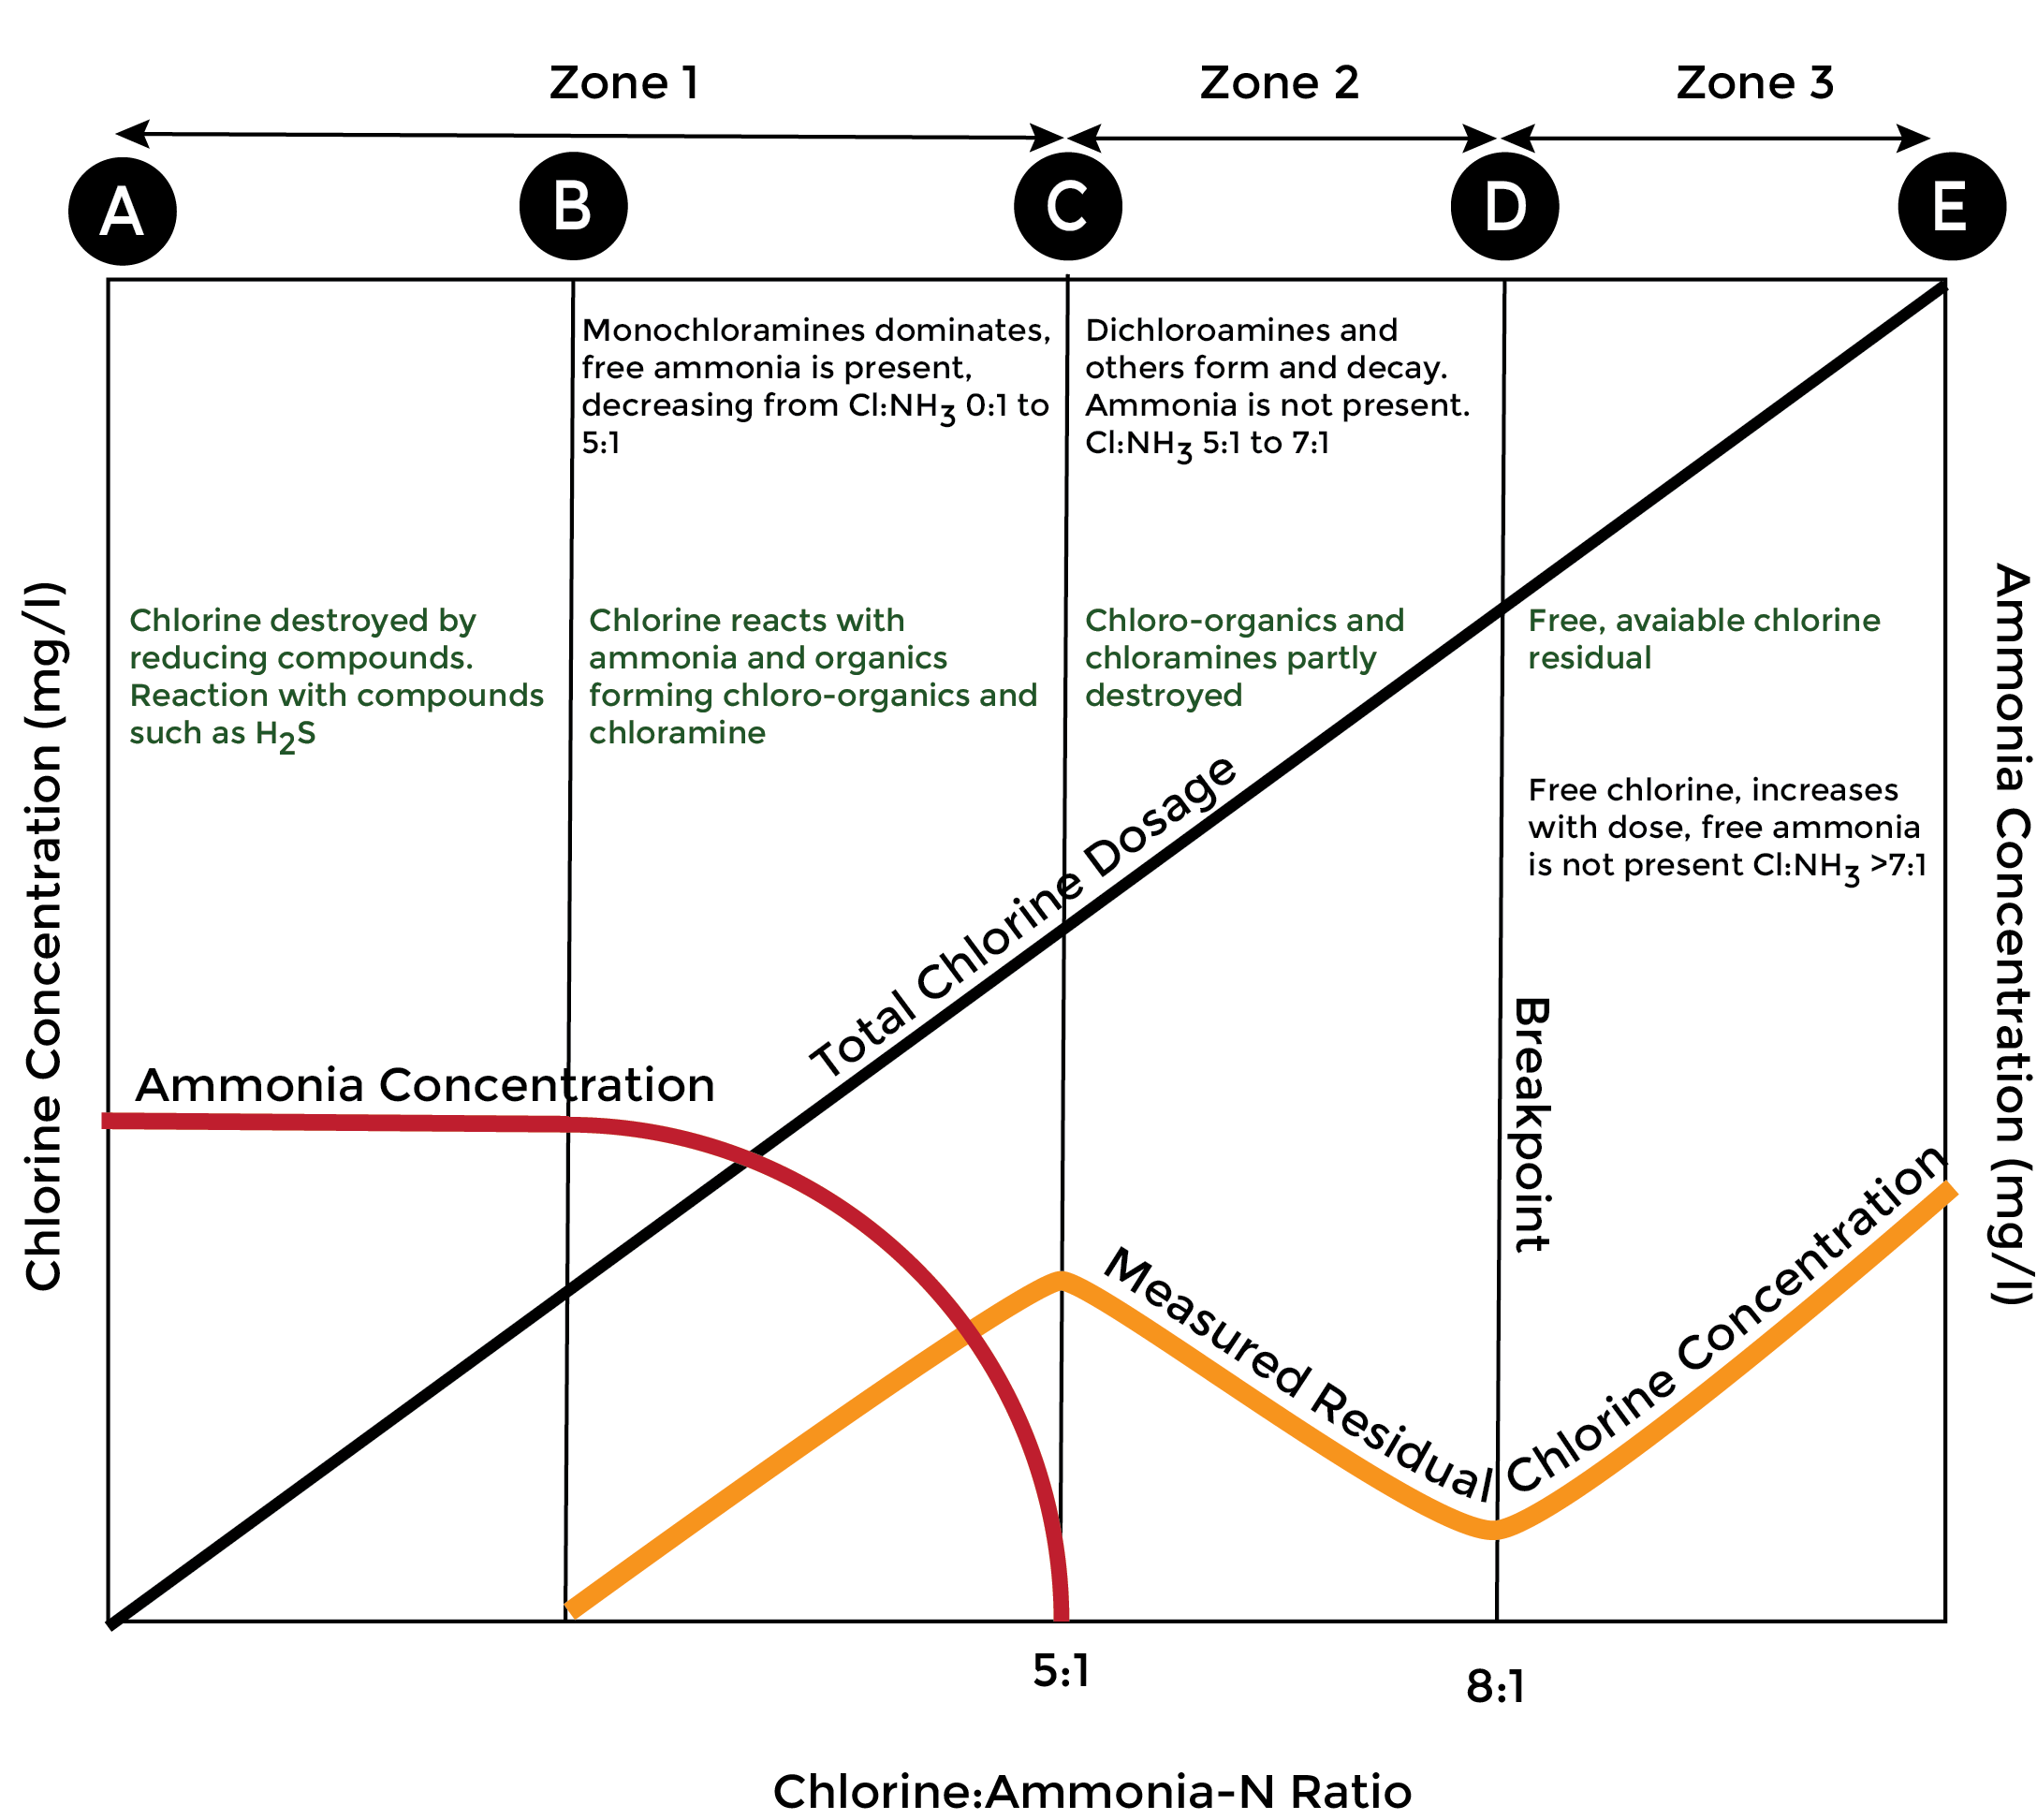
\includegraphics[scale=0.24]{BreakpointChlorination}
			\begin{itemize}
				\item Point A is at the beginning of chlorine application
				\item Between Points A and B, the chlorine dosage produces no residual because of an immediate chlorine demand caused by fast-reacting ions from metal salts and H$_2$S.
				\item Point B is the beginning of the reaction between chlorine and ammonia present
				\item Mono and dichloramines are formed between points B and C
				\item Zone 1 - between points A and C, is the combined zone and has mono and di  chloramines and ammonia.  Mono chloramines is a stable disinfectant while dichloramines is a strong disinfectant but unstable.
				\item After the maximum combined residual is reached (point C), further chlorine doses decrease the residual due to chloramine oxidation to dichloramine, occurring between points C and D.  This is Zone 2 - Breakpoint Zone
				\item Point D represents the breakpoint - the point at which chlorine demand has been satisfied and additional chlorine appears as free residuals
				\item Between points D and E, free available residual chlorine increases in direct proportion to the amount of chlorine applied.  This is Zone 3 which is the free chlorine zone and has hypochlorous acid but no ammonia. \\
			\end{itemize}
			\begin{itemize}
				\item Factors that affect breakpoint chlorination are initial ammonia nitrogen concentration, pH, temperature, and demand exerted by other inorganic and organic species
				\item Weight ratio of chlorine applied to initial ammonia nitrogen must be 8:1 or greater for the breakpoint to be reached. If the weight ratio is less than 8:1, there is insufficient chlorine present to oxidize the chlorinated nitrogen compounds initially formed
				\item When instantaneous chlorine residuals are required, the chlorine needed to provide free available chlorine residuals may be 20 or more times the quantity of ammonia present. Reaction rates are fastest at pH 7-8 and high temperatures
			\end{itemize}


\section{Phosphorous removal}\index{Phosphorous removal}
		\begin{itemize}
		\item Limits related to phosphorous concentrations are commonly found in wastewater treatment facilities' NPDES discharge permits.
		\item Phosphorous removal as part of the treatmnent process accomplishes meeting the NPDES requirement also allows for its recovery for agricultural use.
			\item Phosphorous is very reactive and occurs in nature as phosphate (PO$_4^{\enspace -}$).  
			\item In wastewater phosphorous is present mainly in an inorganic form as orthophosphate (typically about 10 ppm) and as organic phosphate (typically 6 mg/l).
			\item The inorganic phosphate is contributed by detergents and household cleaning products such as soaps
			\item Organic phosphate is contributed by human wastes and food residues as phosphate based molecules play a key role in biological (plant and animals) energy and lifecycles and present in sugars, phospholipids, and nucleotides.  The organic phosphates are decomposed to orthophosphate.
		\end{itemize}
	\vspace{0.3cm}
\subsection{Phosphorous removal methods}\index{Phosphorous removal methods}

\subsubsection{Chemical precipitation method}\index{Chemical precipitation method}

			In the chemical based phosphorous removal method metal salts such as alum and iron salts such as ferric chloride react with soluble phosphate to form solid precipitates that are removed by solids separation processes including clarification and filtration. 
			
			Typically, the phosphate precipitant is applied in both the primary clarifier feed and also just before the secondary clarifier.


			\begin{figure}[h]	
				\begin{center}
					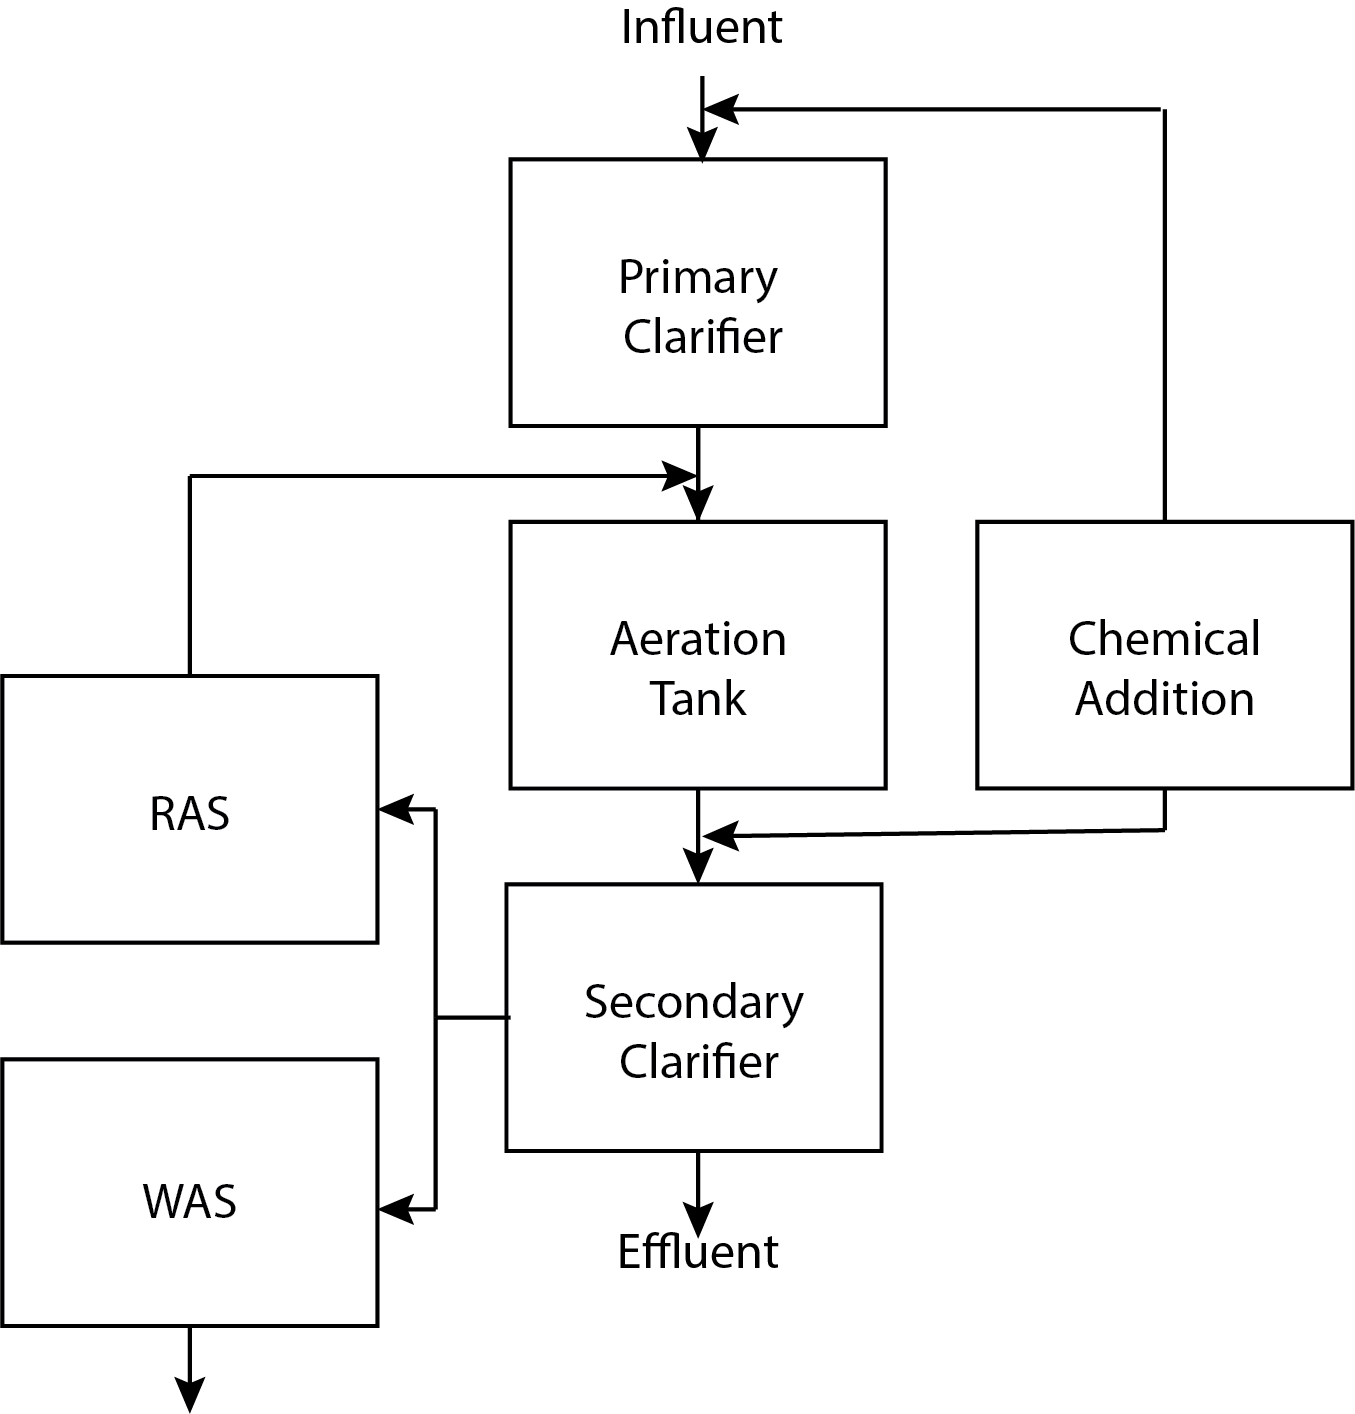
\includegraphics[scale=0.55]{PhosphorousChemical}
					\caption{Chemical removal of phosphorous}
				\end{center}
					\end{figure}
\subsubsection{Enhanced biological phosphorus removal (EBPR)}\index{Enhanced biological phosphorus removal (EBPR)}
				\begin{itemize}
					\item For the removal of phosphorous as part of the activated sludge treatment process:\\
					\begin{itemize}
					\item The process is designed to promote the growth of specific aerobic microorganisms generally known as phosphorus accumulating organisms (PAOs) the activated sludge process.  
					\begin{itemize}
					\item Examples of these bacteria in activated sludge: Acinetobacter, Rhodocyclus
					\item These bacteria have the ability to store substantial quantities of intracellular (inside the bacterial cell) phosphorus.
					\end{itemize}
					
					\item The process is operated by providing alternating anaerobic and aerobic conditions in the aeration basin of the activated sludge treatment process.
				\end{itemize}
				\end{itemize}
			\textbf{EBPR process description:}
				\begin{itemize}
					\item In the anerobic part of the aeration basin, the aerobic bacteria produce VFAs by breaking down organic matter in the influent wastewater.  Thus, the readily biodegradable material - VFAs, is amply available for the PAOs when in the anaerobic environment.  
						\begin{itemize}
							\item Here the PAOs consume the volatile fatty acids (VFAs) produced by the anaerobic fermentation of the organic matter in the anaerobic zone.  Note: This is a fermentation process not anaerobic digestion (in digestion VFAs are destroyed and converted to methane). 
							\item The VFAs are converted into energy rich, carbon based, storable food source.
							\item The energy for this conversion of the VFA into storable food comes from the breakdown of the PAOs polyphosphate reserves.
							\item Ortho phosphate is released during this phase.  
							\item After exposure to enough VFA, the PAOs energy reserves will be depleted and become stressed.  
						\end{itemize}
					\item In the following aerobic phase of the process the PAOs multiply and take up phosphate to replenish the supplies depleted in the anaerobic phase.  
						\begin{itemize}
							\item By oxidizing the carbon reserves built up in the anaerobic phase, PAOs are able to store more phosphate under aerobic conditions than was released under anaerobic conditions because considerably more energy is produced by aerobic oxidation of the stored carbon compounds than was used to store them under anaerobic conditions.
						\end{itemize}
				\end{itemize} 
Eventhough the EPBR requires only a good aeration, its success in removing phosphorous is dependent on the presence of adequate quantities of readily degradable organic material in the secondary influent.
